\documentclass{beamer}
\usepackage[utf8]{inputenc}
\usepackage{gensymb}

\usetheme{Madrid}
\usecolortheme{default}
\usepackage{amsmath,amssymb,amsfonts,amsthm}
\usepackage{txfonts}
\usepackage{tkz-euclide}
\usepackage{listings}
\usepackage{adjustbox}
\usepackage{array}
\usepackage{tabularx}
\usepackage{gvv}
\usepackage{lmodern}
\usepackage{circuitikz}
\usepackage{tikz}
\usepackage{graphicx}

\setbeamertemplate{page number in head/foot}[totalframenumber]

\usepackage{tcolorbox}
\tcbuselibrary{minted,breakable,xparse,skins}



\definecolor{bg}{gray}{0.95}
\DeclareTCBListing{mintedbox}{O{}m!O{}}{%
  breakable=true,
  listing engine=minted,
  listing only,
  minted language=#2,
  minted style=default,
  minted options={%
    linenos,
    gobble=0,
    breaklines=true,
    breakafter=,,
    fontsize=\small,
    numbersep=8pt,
    #1},
  boxsep=0pt,
  left skip=0pt,
  right skip=0pt,
  left=25pt,
  right=0pt,
  top=3pt,
  bottom=3pt,
  arc=5pt,
  leftrule=0pt,
  rightrule=0pt,
  bottomrule=2pt,
  toprule=2pt,
  colback=bg,
  colframe=orange!70,
  enhanced,
  overlay={%
    \begin{tcbclipinterior}
    \fill[orange!20!white] (frame.south west) rectangle ([xshift=20pt]frame.north west);
    \end{tcbclipinterior}},
  #3,
}
\lstset{
    language=C,
    basicstyle=\ttfamily\small,
    keywordstyle=\color{blue},
    stringstyle=\color{orange},
    commentstyle=\color{green!60!black},
    numbers=left,
    numberstyle=\tiny\color{gray},
    breaklines=true,
    showstringspaces=false,
}
%------------------------------------------------------------
%This block of code defines the information to appear in the
%Title page
\title %optional
{2.8.15}
\date{September 3 , 2025}


\author 
{Kartik Lahoti - EE25BTECH11032}



\begin{document}


\frame{\titlepage}
\begin{frame}{Question}
Find the position vector of a point $\vec{A}$ in space such that $\vec{OA}$ is inclined at $60\degree$ with $\vec{OX}$ and $45\degree$ to $\vec{OY}$ and $\mydet{\vec{OA}} = 10 $units.
\end{frame}



\begin{frame}{Theoretical Solution}
Given,
Let $\vec{A} - \vec{O}$ be represented as $\vec{R}$
\begin{align}
    \norm{\vec{R}} = 10 \text{ , Angle with } x\text{-axis} = 60\degree \text{ and } y\text{-axis } = 45\degree
\end{align}

\end{frame}

\begin{frame}{Theoretical Solution}

\begin{align}
    \vec{R} = \norm{\vec{R}} \vec{m}
\end{align}
where, let $\vec{m}$ be the unit vector in direction of $\vec{R}$. 


\begin{align}
    \vec{m} = \myvec{\cos(60\degree) \\ \cos(45\degree) \\ m_3 }
\end{align}

\begin{align}
    \vec{m}^{\top}\vec{m} = 1
\end{align}
\end{frame}
\begin{frame}{Theoretical Solution}
  \begin{align}
    \cos^2(60\degree) + \cos^2(45\degree) + m_3^2 &= 1 \\ 
    m_3 &=\pm \frac{1}{2}  
\end{align}

\begin{align}
    \therefore \vec{R} = 10\myvec{\frac{1}{2} \\ \frac{1}{\sqrt{2}} \\ \pm \frac{1}{2}}
\end{align}
\end{frame}
\begin{frame}{Theoretical Solution}
Hence , 
\begin{align}
    \vec{A}_1 = \myvec{5 \\ 5\sqrt{2} \\ +5} \text{ and } \vec{A}_2 = \myvec{5 \\ 5\sqrt{2} \\ -5} 
\end{align}
are the position vector for point $\vec{A}$
  
\end{frame}
\begin{frame}[fragile]
    \frametitle{C Code (1) }

    \begin{lstlisting}

#include <math.h>
double calc(double l , double m)
{
    double n = sqrt(1 - pow(l,2) - pow(m,2));
    return n ;
}

    \end{lstlisting}
\end{frame}



\begin{frame}[fragile]
    \frametitle{C Code (2)}
    \begin{lstlisting}
    
void linegen(double *X, double *Y , double *Z , double *A , double *B , int n , int m )
{
    double temp[m] ; 
    for (int i = 0 ; i < m ; i++)
    {
        temp [ i ] = (B[i]- A[i]) /(double) n ; 
    }
    for (int i = 0 ; i <= n ; i++ )
    {
        X[i] = A[0] + temp[0] * i ; 
        Y[i] = A[1] + temp[1] * i ;
        Z[i] = A[2] + temp[2] * i ; 
    }
}

\end{lstlisting}
\end{frame}

\begin{frame}[fragile]
    \frametitle{Python Code - Using Shared Object}
    \begin{lstlisting}
import ctypes
import numpy as np
import matplotlib.pyplot as plt
handc1 = ctypes.CDLL("./func.so")

handc1.calc.argtypes=[
    ctypes.c_double,
    ctypes.c_double
]
l = np.cos(np.deg2rad(60))
m = np.cos(np.deg2rad(45))

handc1.calc.restype = ctypes.c_double

n = handc1.calc(l , m)
\end{lstlisting}
\end{frame}


\begin{frame}[fragile]
    \frametitle{Python Code - Using Shared Object}
    \begin{lstlisting}

def line_cre(P: np.ndarray , Q: np.ndarray, str):
    handc2 = ctypes.CDLL("./line_gen.so")

    handc2.linegen.argtypes = [
        ctypes.POINTER(ctypes.c_double),
        ctypes.POINTER(ctypes.c_double),
        ctypes.POINTER(ctypes.c_double),
        ctypes.POINTER(ctypes.c_double),
        ctypes.POINTER(ctypes.c_double),
        ctypes.c_int , ctypes.c_int
    ]

    handc2.linegen.restype = None
    


\end{lstlisting}
\end{frame}
\begin{frame}[fragile]
    \frametitle{Python Code - Using Shared Object}
    \begin{lstlisting}
    n = 200
    X_l = np.zeros(n,dtype=np.float64)
    Y_l = np.zeros(n,dtype=np.float64)
    Z_l = np.zeros(n,dtype=np.float64)
    handc2.linegen (
        X_l.ctypes.data_as(ctypes.POINTER(ctypes.c_double)),
        Y_l.ctypes.data_as(ctypes.POINTER(ctypes.c_double)),
        Z_l.ctypes.data_as(ctypes.POINTER(ctypes.c_double)),
        P.ctypes.data_as(ctypes.POINTER(ctypes.c_double)),
        Q.ctypes.data_as(ctypes.POINTER(ctypes.c_double)),
        n,2
    )
    ax.plot([X_l[0],X_l[-1]],[Y_l[0],Y_l[-1]],[Z_l[0],Z_l[-1]],str)

    \end{lstlisting}
\end{frame}

\begin{frame}[fragile]
    \frametitle{Python Code - Using Shared Object}
    \begin{lstlisting}

A1 = 10 * np.array([[l],[m],[n]],dtype=np.float64).reshape(-1,1)
A2 = 10 * np.array([[l],[m],[-n]], dtype= np.float64).reshape(-1,1)
B = np.array([[0],[0],[0]]).reshape(-1,1)
fig = plt.figure()
ax = fig.add_subplot(111,projection="3d")

line_cre(A1,B,"g-")
line_cre(A2,B,"r-")

coords = np.block([[A1,A2,B]])
ax.scatter(coords[0,:],coords[1,:],coords[2,:])
vert_labels = [r'$A_1$',r'$A_2$','O']


\end{lstlisting}
\end{frame}

\begin{frame}[fragile]
    \frametitle{Python Code - Using Shared Object}
    \begin{lstlisting}
for i, txt in enumerate(vert_labels):
    if (coords[0,i] == 0 ) :
        ax.text(coords[0,i], coords[1,i] , coords[2,i],txt , ha='center', va = 'bottom')
    else :
        ax.text(coords[0,i], coords[1,i] , coords[2,i],f'{txt}\n({coords[0,i]:.1f}, {coords[1,i]:.1f}, {coords[2,i]:.1f})',ha='center', va = 'bottom')
ax.scatter(coords[0,2], coords[1,2], coords[2,2], color="b", label="O : ORIGIN")
ax.legend(loc = "best")
ax.set_xlabel('$x$')
ax.set_ylabel('$y$')
ax.set_zlabel('$z$')
\end{lstlisting}
\end{frame}

\begin{frame}[fragile]
    \frametitle{Python Code - Using Shared Object}
    \begin{lstlisting}
ax.grid()
ax.set_xlim([-2, 7])
ax.set_ylim([-2,8])
ax.set_zlim([-6,6])
plt.title("Fig:2.8.15")
#ax.set_box_aspect([1,1,1])

fig.savefig("../figs/vector1.png")
fig.show()

#plt.savefig('figs/triangle/ang-bisect.pdf')
#subprocess.run(shlex.split("termux-open figs/triangle/ang-bisect.pdf"))

\end{lstlisting}
\end{frame}




\begin{frame}[fragile]
    \frametitle{Python Code}
    \begin{lstlisting}
import math
import sys
sys.path.insert(0, '/home/kartik-lahoti/matgeo/codes/CoordGeo')
import numpy as np
import numpy.linalg as LA
import matplotlib.pyplot as plt
import matplotlib.image as mpimg

from line.funcs import *
#from triangle.funcs import *
#from conics.funcs import circ_gen


#if using termux
#import subprocess
#import shlex


\end{lstlisting}
\end{frame}

\begin{frame}[fragile]
    \frametitle{Python Code }
    \begin{lstlisting}

l = np.cos(np.deg2rad(60))
m = np.cos(np.deg2rad(45))
n = np.sqrt(1 - l**2 - m**2)

A1 = 10 * np.array([l,m,n]).reshape(-1,1)
A2 = 10 * np.array([l,m,-n]).reshape(-1,1)
O = np.array([0,0,0]).reshape(-1,1)

def plot_it(P,Q,str):
    x_l = line_gen_num(P,Q,20)
    ax.plot(x_l[0,:],x_l[1,:],x_l[2,:] , str )

fig = plt.figure()
ax = fig.add_subplot(111,projection = "3d")

plot_it(A1,O,"g-")
plot_it(A2,O,"r-")

\end{lstlisting}
\end{frame}

\begin{frame}[fragile]
    \frametitle{Python Code }
    \begin{lstlisting}
coords = np.block([[A1,A2,O]])
plt.scatter(coords[0,:],coords[1,:],coords[2,:])
vert_labels = [r'$A_1$',r'$A_2$','O']
for i, txt in enumerate(vert_labels):
    if (coords[0,i] == 0 ) :
        ax.text(coords[0,i], coords[1,i] , coords[2,i],txt , ha='center', va = 'bottom')
    else :
        ax.text(coords[0,i], coords[1,i] , coords[2,i],f'{txt}\n({coords[0,i]:.1f}, {coords[1,i]:.1f}, {coords[2,i]:.1f})',ha='center', va = 'bottom')

ax.scatter(coords[0,2], coords[1,2], coords[2,2], color="b", label="O : ORIGIN")
ax.legend(loc = "best")
\end{lstlisting}
\end{frame}


\begin{frame}[fragile]
    \frametitle{Python Code }
    \begin{lstlisting}

ax.set_xlabel('$x$')
ax.set_ylabel('$y$')
ax.set_zlabel('$z$')
ax.grid()
ax.set_xlim([-2, 7])
ax.set_ylim([-2,8])
ax.set_zlim([-6,6])
plt.title("Fig:2.8.15")
#ax.set_box_aspect([1,1,1])

fig.savefig("../figs/vector2.png")
fig.show()
#.run(shlex.split("termux-open figs/triangle/ang-bisect.pdf"))

    \end{lstlisting}
\end{frame}


\begin{frame}{Plot}
    \centering
    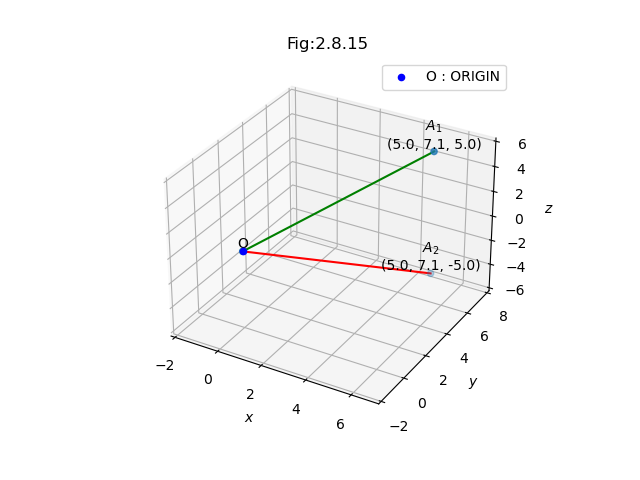
\includegraphics[width=\columnwidth, height=0.8\textheight, keepaspectratio]{figs/vector1.png}   
\end{frame}


\end{document}
